\begin{figure}[h!]
\centering
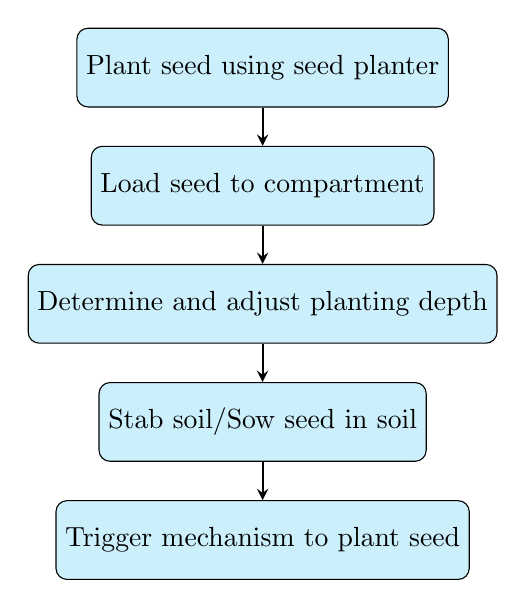
\begin{tikzpicture}[node distance=1.5cm]

\tikzstyle{startstop} = [rectangle, rounded corners, minimum width=3cm, minimum height=1cm,text centered, draw=black, fill=cyan!20]
\tikzstyle{arrow} = [thick,->,>=stealth]

\node (start) [startstop] {Plant seed using seed planter};
\node (load) [startstop, below of=start] {Load seed to compartment};
\node (depth) [startstop, below of=load] {Determine and adjust planting depth};
\node (stab) [startstop, below of=depth] {Stab soil/Sow seed in soil};
\node (trigger) [startstop, below of=stab] {Trigger mechanism to plant seed};

\draw [arrow] (start) -- (load);
\draw [arrow] (load) -- (depth);
\draw [arrow] (depth) -- (stab);
\draw [arrow] (stab) -- (trigger);

\end{tikzpicture}
\caption{Minimum planting layout in Session 8}
\label{fig:planting_flowchart}
\end{figure}
